\documentclass[11pt]{beamer}
\usetheme{Warsaw}
\usepackage[utf8]{inputenc}
\usepackage{amsmath}
\usepackage{amsfonts}
\usepackage{amssymb}
\usepackage{graphicx}

\graphicspath{{images/}}

%\begin{figure}[h!]
%\begin{center}
%\includegraphics[scale = 0.5]{exercise_3_11_a.png}
%\caption{SAS Output for $X^2$ and $G^2$ tests}
%\end{center}
%\end{figure}

\usepackage[english]{babel}
\usepackage{comment}
\usepackage{textcomp}
\usepackage{color}
\usepackage{listings}   
\lstset{language=R,
    basicstyle=\fontsize{5}{7}\ttfamily,
    %stringstyle=\color{DarkGreen},
    otherkeywords={0,1,2,3,4,5,6,7,8,9},
    morekeywords={TRUE,FALSE},
    deletekeywords={data,frame,length,as,character},
    keywordstyle=\color{blue},
    %commentstyle=\color{DarkGreen},
}                



\setbeamerfont{itemize/enumerate}{size=8pt}

\author{Collin Nolte}
\title[FDR]{Multiple Hypothesis Testing and False Discovery Rates}
\setbeamercovered{transparent} 
\setbeamertemplate{navigation symbols}{} 
%\logo{} 
%\institute{} 
%\subtitle{AMCS Seminar}
\date{March 6, 2018} 

\begin{document}

\begin{frame}
\titlepage
\end{frame}

\begin{frame}
\frametitle{Table of Contents}
\tableofcontents
\end{frame}

\section{General Hypothesis Testing}
\subsection{The Null Hypothesis}



\begin{frame}
\frametitle{The Null Hypothesis}
{

\begin{itemize}
\item Formally, a (usually dichotomous) statement that is testable on the basis of observing a process modeled by a set of random variables, or a random event \\
\item Testable in that we can use observed data to quantify the strength of the statement, given observed data or outcome \\
\item Can be used to test a particular statement of interest, or used (in the same manner) as a set of diagnostics for variable coefficients in a  regression model 

\item The alternate hypothesis is usually a negation of the null, although could be one-sided
\begin{align*}
Y = X \beta, \quad \beta \in \mathbb{R}^p \qquad \qquad 	\begin{cases}
H_{0_{(i)}}&: \beta_i = 0 \\
H_{A_{1(i)}}&: \beta_i \not= 0 \\
H_{A_{2(i)}}&: \beta_i > 0
\end{cases}
\end{align*}
\end{itemize}
}
\end{frame}

%%%%%%%%%%%%%%%%%%
\subsection{p-values}

\begin{frame}
\frametitle{p-values}
{
\begin{itemize}
\item The quantification of the strength of the null hypothesis is the p-value, which is the probability of the observed data, assuming that the null hypothesis is true \\
\item Suppose we have observed data $x$ from a random process with standard error $SE$, and we hypothesize that it's true value is equal to $\hat{x}_0$, that is, $E(x) = \hat{x}$. By the central limit theorem, we have
\begin{align*}
\frac{x - \hat{x}}{SE} \stackrel{def}{=} z \sim N(0,1) \qquad \qquad 
\begin{cases}
H_0: x - \hat{x} = z = 0 \\
H_A: x - \hat{x} = z \not= 0
\end{cases}
\end{align*}
\end{itemize}
}
\end{frame}

\begin{frame}
\frametitle{p-values cont}
{
We can then consider the value of $\frac{x - \hat{x}}{SE}$ in the context of its assumed distribution

\begin{figure}
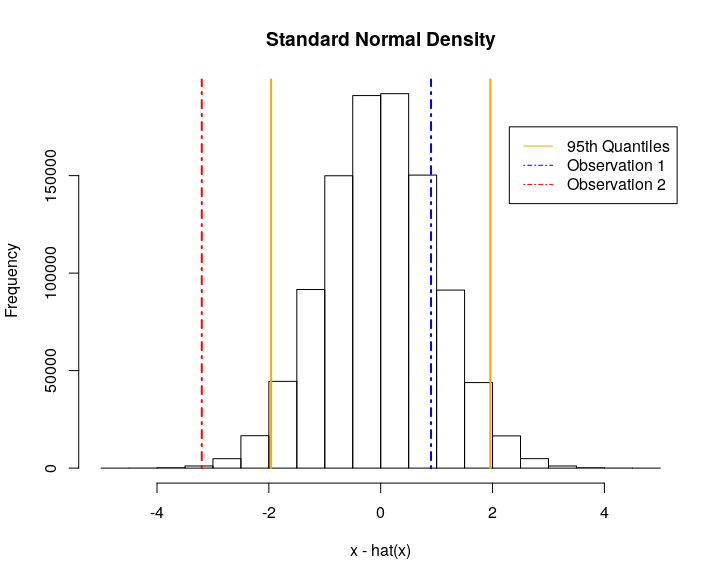
\includegraphics[scale = 0.4]{normalPlot.png} \\
\end{figure}
}
\end{frame}

\subsection{Types of Errors}

\begin{frame}
\frametitle{Type I and Type II Errors}

\begin{itemize}
\item p-value represents a probability, rather than certainty \\
\item By chance alone, uninteresting outcomes could be considered significant \\
\item The Type 1 error rate is called the significance level, the probability of rejecting a null hypothesis when it is true \\
\item Similarly, the power of a test is the probability of not committing a type II error, or falsely determining significance when there is none
\end{itemize}

\begin{center}
\begin{tabular}{c| c c }
\hline
& \multicolumn{2}{c}{Null Hypothesis} \\[3pt]
& $H_0$ True & $H_0$ False \\
\hline 
$H_0$ Rejected & Type 1 Error & Correct  \\[2pt]
$H_0$ Not Rejected & Correct & Type II Error \\[1pt]
\hline
\end{tabular}
\end{center}
\end{frame}

\section{The Problem of Multiple Comparison}

\begin{frame}
\frametitle{Refresher in Probability}
{
\begin{itemize}
\item For events $A$ and $B$, we have (Bayes Rule) that
\begin{align*}
P(B|A) &= \frac{P(A \cap B)}{P(A)} \\[6pt]
P(A \cap B) &= P(B|A)P(A) \leq P(B)P(A)
\end{align*}
where, under independence of events, $P(B|A) = P(B)$ \\
\item In general, then, the assumption that $A$ and $B$ are independent results in a larger probability of them both occurring than if they had non-empty intersection
\end{itemize}
}
\end{frame}

\subsection{Family-Wise Error Rates}

\begin{frame}
\frametitle{Type 1 Error for Multiple Tests}
{
\begin{itemize}
\item Suppose, then, that we have $k$ sets of hypothesis tests, with a predetermined Type 1 Error rate (significance level) of $\alpha$ \\
\item The probability that any particular test does incorrectly reject a true null hypothesis is $1 - \alpha$ \\
\item Under the conservative assumption that each hypothesis test is in independent of one another, the probability of $k$ tests not incorrectly rejecting a true null is
\begin{align*}
P(\text{no Type 1 errors}) &= \prod^k (1 - \alpha) = (1-\alpha)^k
\end{align*}
\item Consider a situation in which $k = 20$, with predetermined significance of $\alpha = 0.5$. The probability of committing no errors now becomes $(1 - 0.95)^{20} = 0.3584$ \\
\end{itemize}
}
\end{frame}

\begin{frame}
\frametitle{Family-Wise Error Rates}
{
\begin{itemize}
\item This can be restated as the Family-Wise Error Rate (FWER), or the probability of committing at least one error
\begin{align*}
FWER &= P(\text{at least 1 error}) \\[4pt]
&= 1 - P(\text{no errors}) \\[4pt]
&= 1 - \prod_{i=1}^k (1 - \alpha) \\[4pt]
&= 1 - (1 - \alpha)^k
\end{align*} 
\item We can use this to specify $\alpha$ to control our FWER:
\begin{align*}
\alpha = 1 - (1 - FWER)^{\frac{1}{k}}
\end{align*}
\end{itemize}
}
\tiny{Slide modified from BIOS 5720, Spring 2017}
\end{frame}

\subsection{Corrections and Procedures}

\begin{frame}
\frametitle{Corrections and procedures}
{\small
\begin{itemize}
\item Sidac Correction, holds under independence, otherwise conservative
\begin{align*}
\alpha = 1 - (1 - FWER)^{1/k}
\end{align*}
\item Bonferroni Correction modifies nominal value of $\alpha$, dependent on $k$
\begin{align*}
P(\text{Type 1 Error}) &= P\left( \bigcup_{i=1}^k z_i \leq \frac{\alpha}{k} \right) \\[6pt]
&\leq \sum_{i=1}^k P \left(  z_i \leq \frac{\alpha}{k} \right) \\[6pt]
&\leq k \left( \frac{\alpha}{k} \right) = \alpha
\end{align*}
\item Alternatively, we could choose a different partition of $\alpha$, the modifications can be thought of as weights 'spent' over each of the $k$ tests
\end{itemize}
\tiny{Slide modified from BIOS 5720, Spring 2017}
}
\end{frame}

\subsection{Large Feature Data}

\begin{frame}
\frametitle{Issues}
{
\begin{itemize}
\item These tests tend to be overly conservative \\
\item What if $k$ is really really big?
\item Microarray gene data can have anywhere from 5,000 to 50,000 genes on which we are conducting a hypothesis
\item We can no longer make crude adjustments and expect to find results
\end{itemize}
}
\end{frame}

\begin{frame}
\frametitle{West Gene Dataset Example, ER Status}
{
\begin{itemize}
\item West data set is a collection of 49 breast cancer tissue samples measuring the expression level of 7129 genes \\
\item The samples were classified according to it's estrogen receptor (ER) status, a marker explaining several characteristics about the tumor \\
\item Goal was to identify a set of genes that may be significant in determining the classification of a sample \\
\item For each gene, significance was tested by comparing the mean expression of the gene in subjects who were $ER_+$ against those who were $ER_-$ \\
\item The null hypothesis is that an individual gene is not significant, i.e., there is no difference in mean expression level, i.e
\begin{align*}
H_0: \mu_{ER_+} = \mu_{ER_-} \quad \Rightarrow \quad H_0:  \mu_{ER_+} - \mu_{ER_-} = 0
\end{align*}
\end{itemize}
}
\end{frame}

\begin{frame}[fragile]
\frametitle{West Gene Dataset}
{
\begin{lstlisting}
## Create vector for ER status for each sample (1 = ER+, 0 = ER-)
er <- clinical$ER
table(er)
er
 0  1 
24 25 

## Perform two-sample t-tests for each gene and save all p-values
pval <- NULL
stat <- NULL
m <- nrow(chip.norm)
for(i in 1:m) {
   result <- t.test(chip.norm[i,] ~ er)
   pval <- c(pval, result$p.value)
   est <- result$estimate
   stat <- c(stat, est[2] - est[1])
}

## Number of p-values significant at the 5% level
> sum(pval < 0.05)
[1] 1325

## Bonferroni adjustment
> sum(pval < 0.05 / length(pval))
[1] 26
\end{lstlisting}
}
\end{frame}

\begin{frame}
\frametitle{West Gene Data Continued}
\begin{columns}
\column{0.5\textwidth}

\begin{figure}
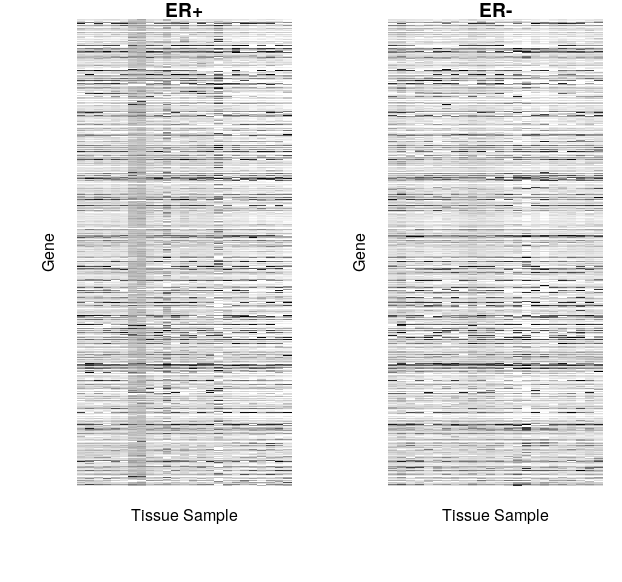
\includegraphics[scale = 0.3]{geneImage.png} 
\end{figure}

\column{0.5\textwidth}

\begin{figure}
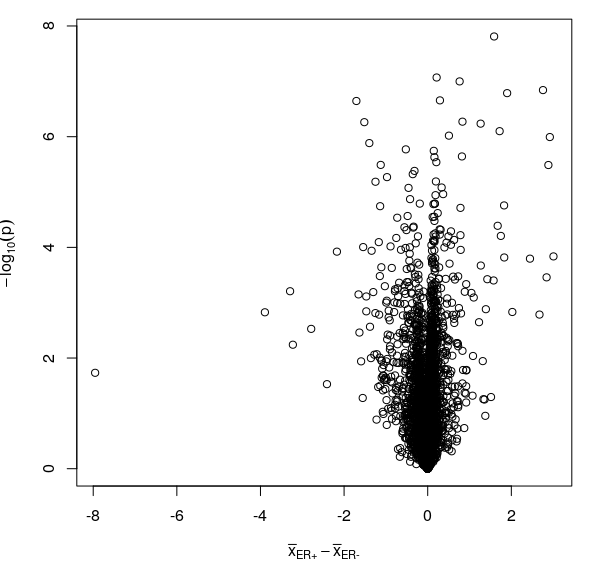
\includegraphics[scale = 0.3]{volcano.png} 
\end{figure}

\end{columns}
\tiny{Images and code modified from BIOS 6720, Spring 2018}
\end{frame}

\section{False Discovery Rates}

\begin{frame}
\frametitle{False Discovery Rates}
{
\begin{itemize}
\item By chance, we expect $\alpha \%$ of the $M$ genes to be considered significant \\
\item In table below, $V$ now represents the occurence of a type 1 error amongst the $M$ tests, and $P(V \geq 1)$ would be our FWER. This value is unobserved
\item $R$ represents the total number of genes declared significant, regardless of the true value. This value is observed and known
\end{itemize}

\begin{center}
\begin{tabular}{c| c c c}
\hline
& \multicolumn{3}{c}{Null Hypothesis} \\[3pt]
& $H_0$ True & $H_0$ False & Total\\
\hline 
$H_0$ Rejected & V & S & R \\[2pt]
$H_0$ Not Rejected & U & T  & M-R \\[1pt]
\hline
Total & $M_0$& $M_1$& M\\
\hline
\end{tabular}
\end{center}
}
\end{frame}

\begin{frame}
\frametitle{False Discovery Rates}
{
\begin{itemize}
\item Define the False Discovery Rate (FDR) to be 
\begin{align*}
FDR = E(V/R)
\end{align*}
\item Regardless of independence or the distribution of the p-values, it holds that
\begin{align*}
FDR = E(V/R) \leq \frac{V+U}{M} \alpha = \frac{M_0}{M} \alpha \leq \alpha
\end{align*}
Hence, controlling for FDR effectively allows us to control for $\alpha$. However, this is NOT the FWER
\end{itemize}
\begin{center}
\begin{tabular}{c| c c c}
\hline
& \multicolumn{3}{c}{Null Hypothesis} \\[3pt]
& $H_0$ True & $H_0$ False & Total\\
\hline 
$H_0$ Rejected & V & S & R \\[2pt]
$H_0$ Not Rejected & U & T  & M-R \\[1pt]
\hline
Total & $M_0$& $M_1$& M\\
\hline
\end{tabular}
\end{center}
}
\end{frame}

\begin{frame}
\frametitle{Sources}
{
\begin{itemize}
\item Course notes BIOS 5270 \\
\item Course notes BIOS 6270 \\
\item "Elements of Statistical Learning", Chapter 18, Trevor Hastie, Robert Tibshirani, Jerome Friedman. \\
\item "Controlling the False Discovery Rate: a Practical and Powerful Approach to Multiple Testing", Yoav Benjamini, Yosef Hochberg, Jan 1993.
\end{itemize}
}
\end{frame}










\end{document}